\label{sec:vbf-parsigz}

This section describes the background estimation and likelihood fit strategy, which are determined together.

In order to describe the data, we consider three contributions to the \Mbb{} distribution:  
\begin{itemize}
  \item Signal $H\rightarrow b \bar b$ from either VBF or ggF production
  \item Resonant \zjets{} from QCD and EW production
  \item Non-resonant processes dominated by QCD multi-jet production
\end{itemize}

The shapes of the signal and \zjets{} contributions are each parametrized by a Bukin function. The non-resonant background is taken from data using a fit with an analytical function in the \Mbb{} sidebands of the signal regions and control region as described in Section~\ref{sec:vbf-nonres}.
The signal strength is measured with a profile likelihood fit performed
simultaneously for all signal and control regions.  The $Z$ normalization is treated as a nuisance parameter in the fit.  The Higgs mass window, 100 \GeV$<\Mbb<$140\GeV, is blinded for the signal regions.  

\subsubsection{Asimov Dataset}
\label{sec:vbf-asimov}
Asimov dataset is used in this analysis for closure tests and sensitivity study. An Asimov dataset is the sum of the Higgs signal, \zjets{} process and the analytical non-resonant background. The parameterization of Higgs signal and \zjets{} components are described in \ref{sec:vbf-parsigz}. The normalization of the Higgs signal and \zjets{} components is the product of the expected strength and the yield taken from MC prediction. The parameterization of the analytical non-resonant background is described in \ref{sec:vbf-nonres}. The normalization of the non-resonant background is estimated by scaling the number of events of the 0-tag sample by the ratio of the events in the sidebands for the 2- and 0-tag samples. Specifically $B$ is given by $N_{\rm 0~tag, mw}\times \frac{N_{\rm 2~tag, sb}}{N_{\rm 0~tag, sb}}$ where  $N_{\rm 0~tag, mw}$ is the number of events from the 0-tag sample in the Higgs mass window, and $N_{\rm 2(0)~tag, sb}$ is the number of events in the side-band regions for 2(0)-tag sample.

\subsubsection{Parameterization of signal and \zjets{}}



We parameterize the signal and \zjets{} Monte Carlo templates to smooth out the local fluctuations coming from the limited statistics using a histogrammed Bukin function. The MC templates and parametrization of signal and \zjets{} \Mbb{} distributions are shown in Figures~\ref{fig:vbf-sigpar_alt} and \ref{fig:vbf-zpar_alt}. The $\chi^2$ between simulated and fitted distributions are summarized in Table~\ref{tab:sigpar_alt}. In general, the $\Mbb$ distributions for the Higgs signal and \zjets{} are well represented by the Bukin function. The potential bias of using smoothed MC templates is studied in the full profile likelihood fit. Perfect closure is obtained with $\mu_{H}=1$ and $\mu_{Z}=1$, as injected in the Asimov data.  Therefore we conclude that the parameterized templates produce no significant bias.  The likelihood fit is described in detail later in this section.

 
\begin{figure}[htbp]
  \centering    
 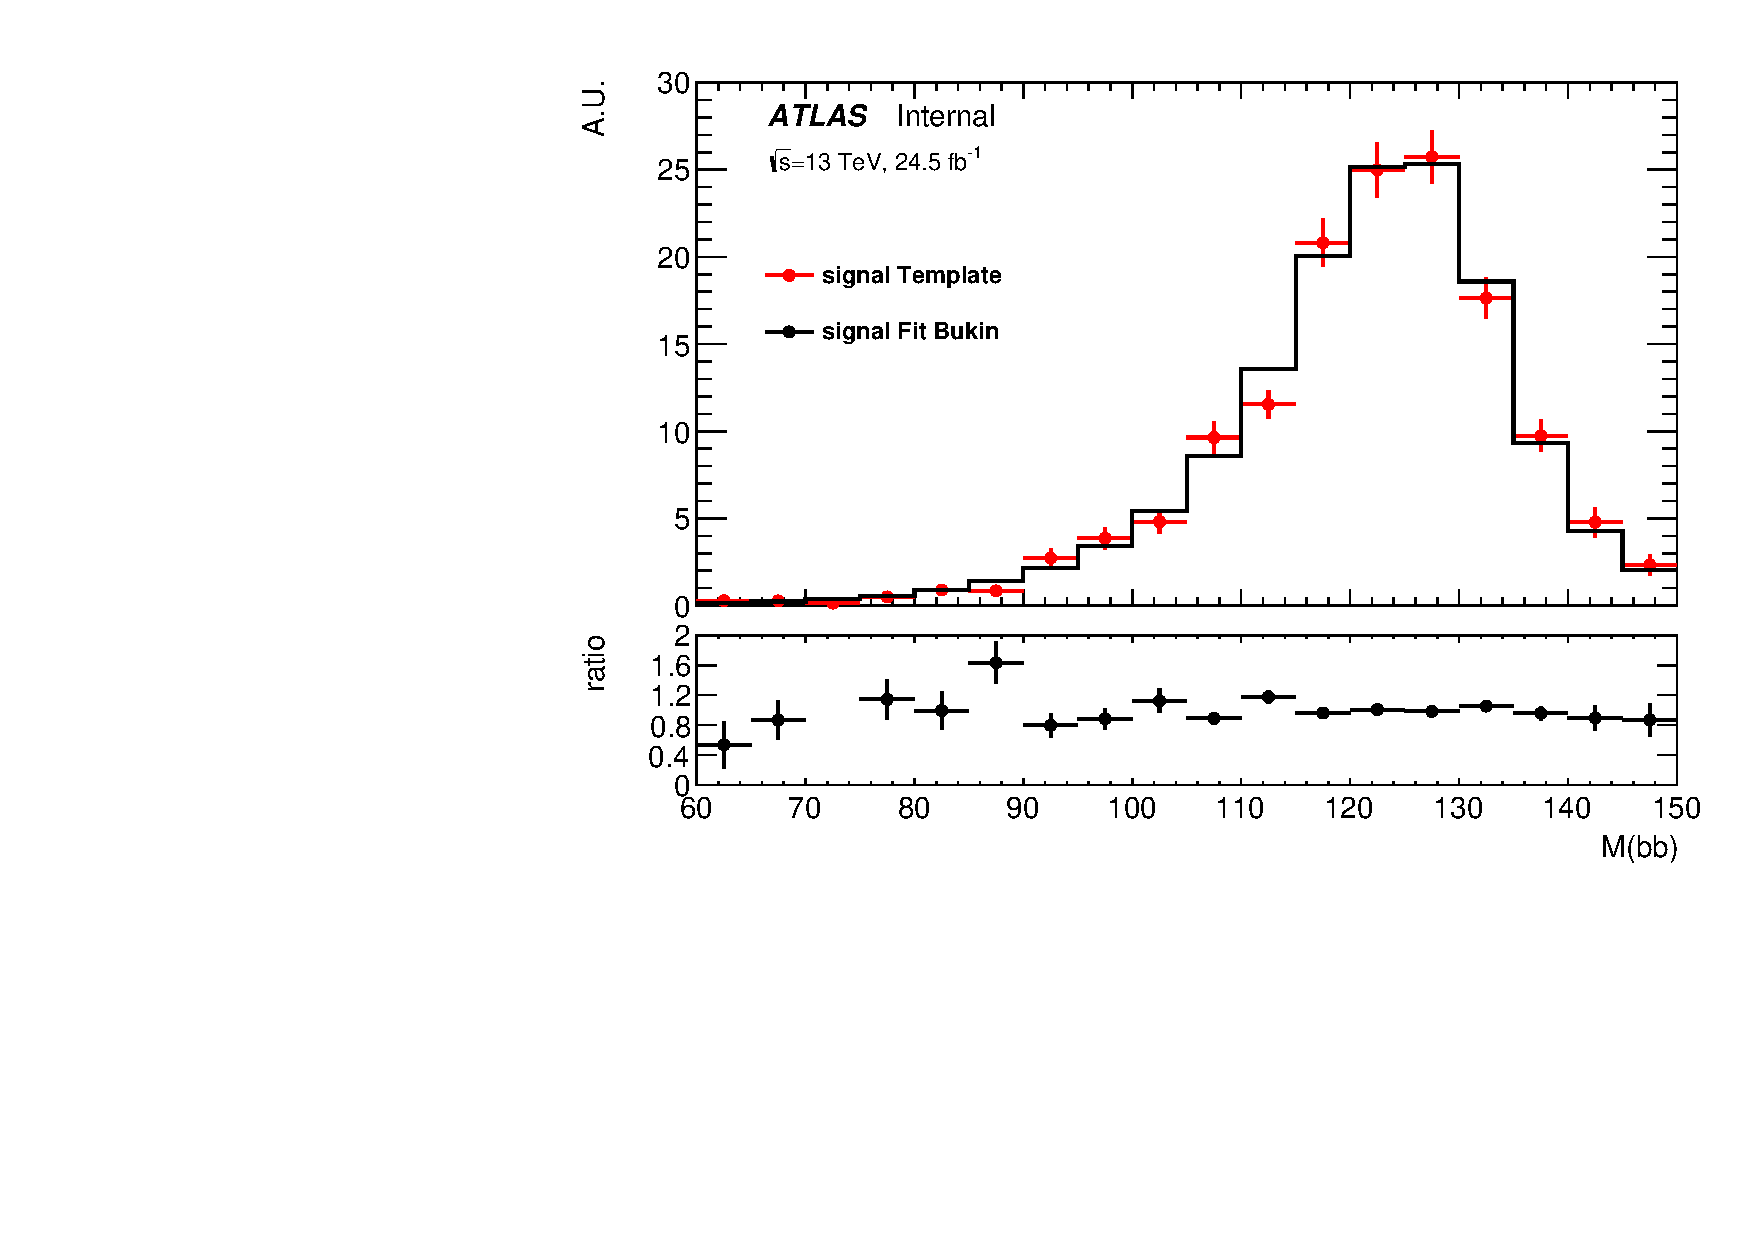
\includegraphics[width=0.24\textwidth]{figures/VBF/sig_2cen_SRI.pdf}
 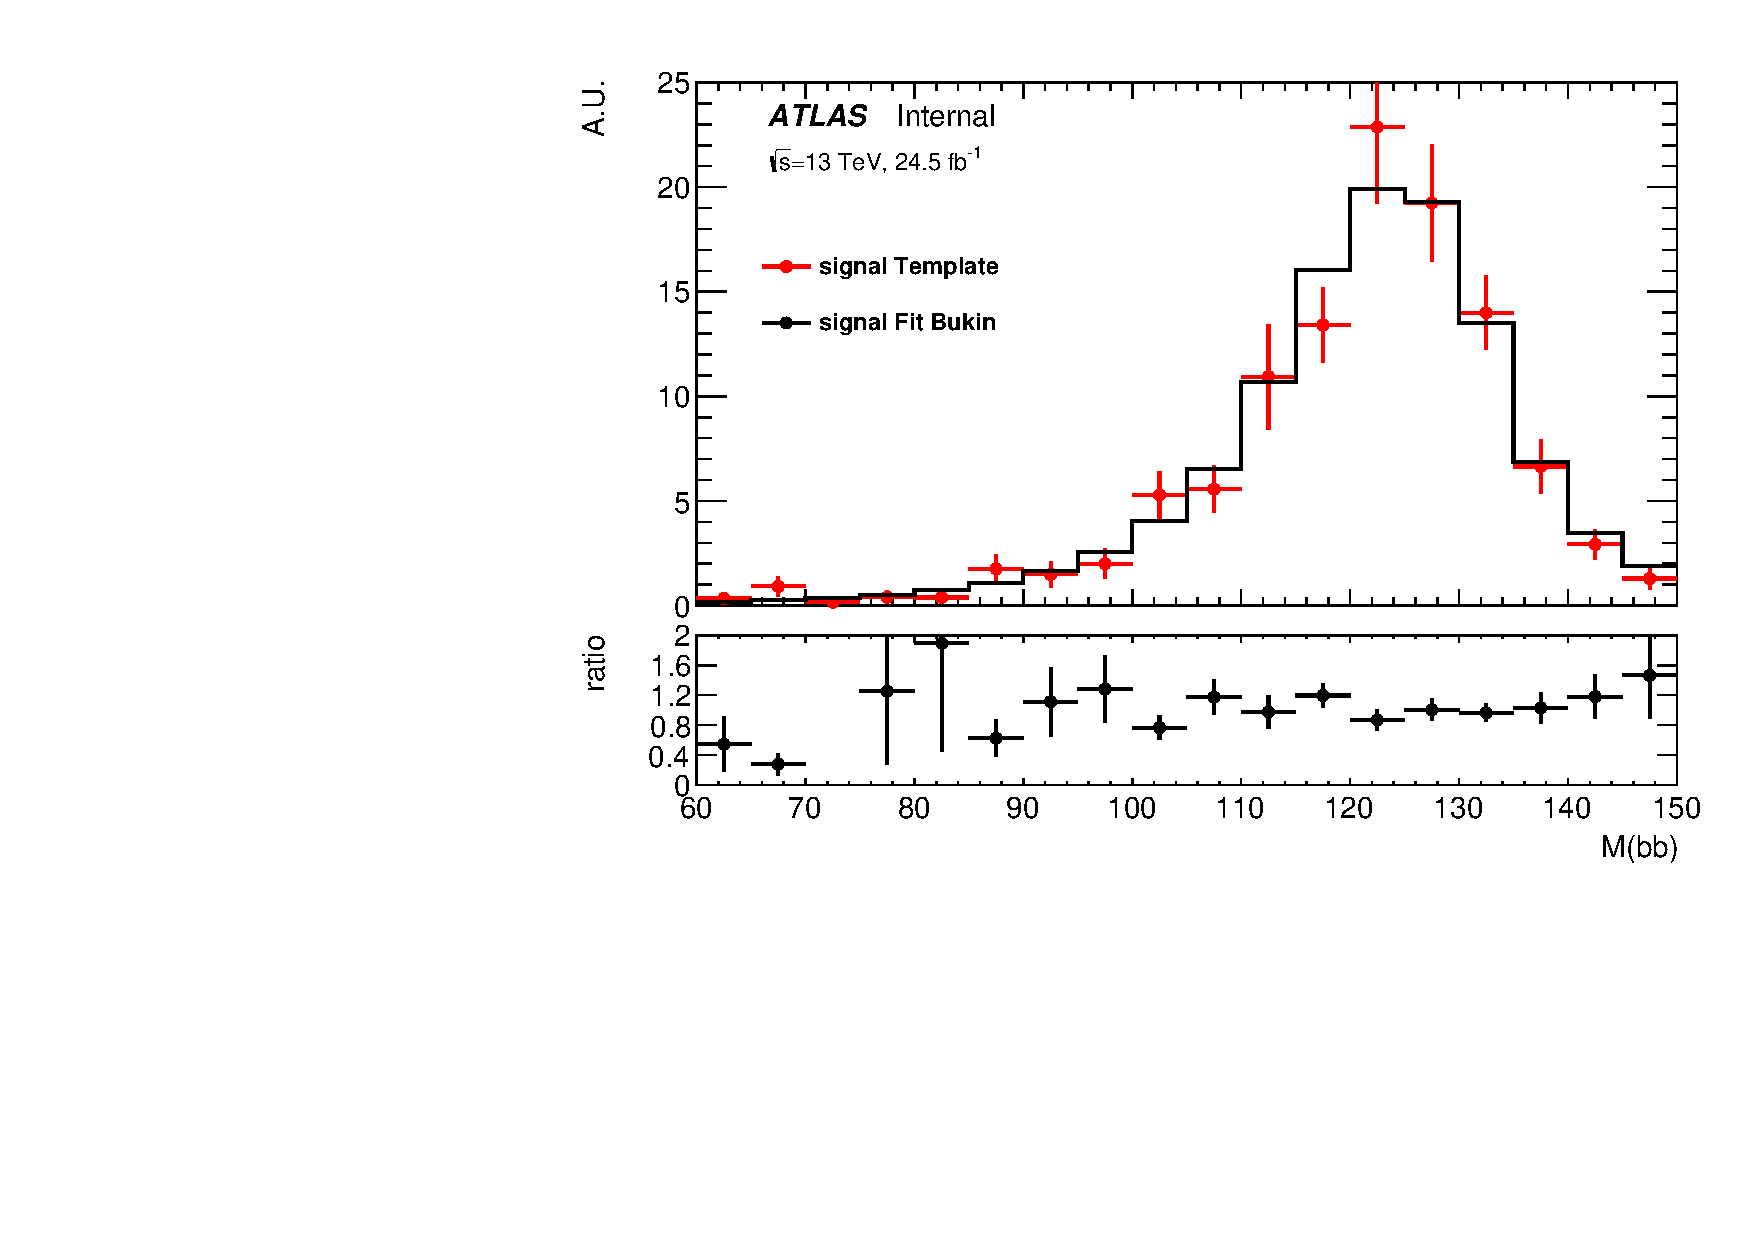
\includegraphics[width=0.24\textwidth]{figures/VBF/sig_2cen_SRII.pdf}\\
 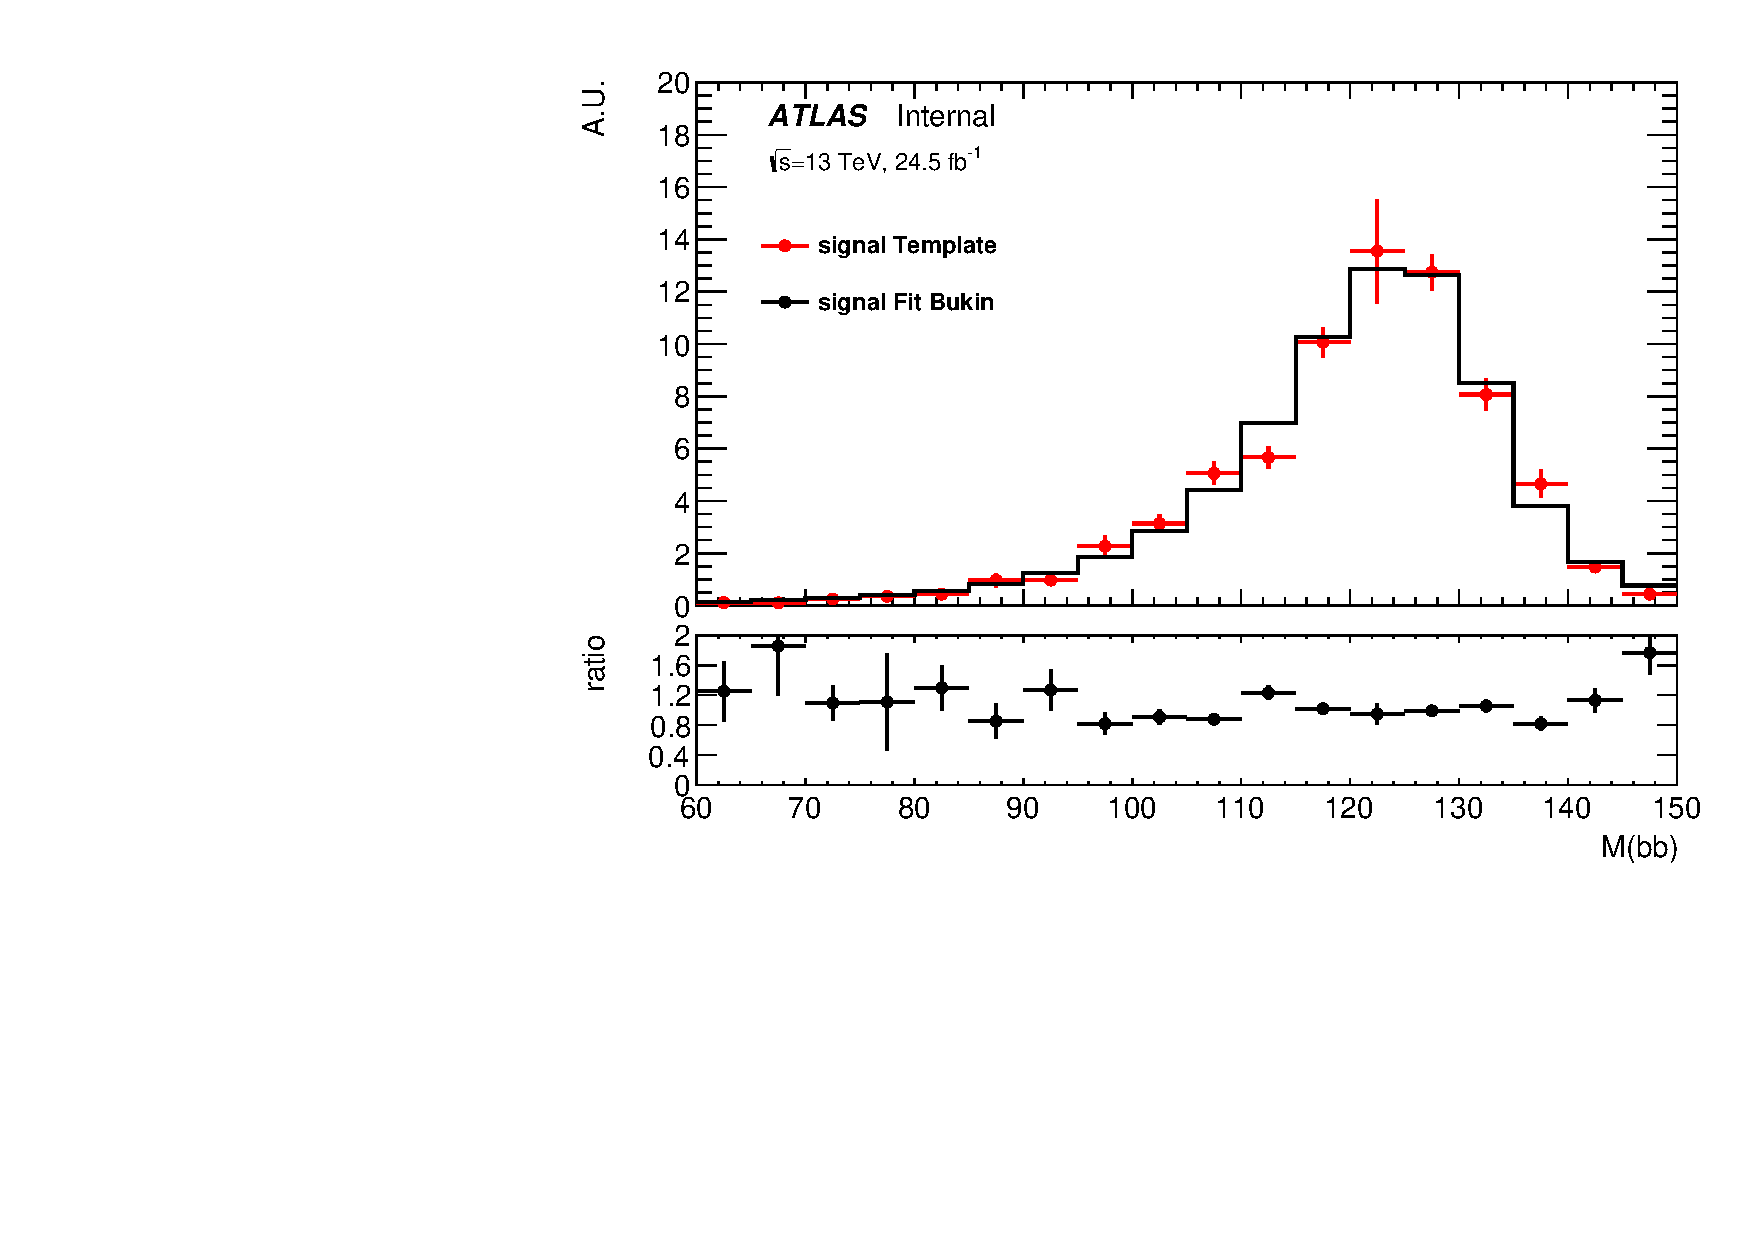
\includegraphics[width=0.24\textwidth]{figures/VBF/sig_4cen_SRI.pdf}
 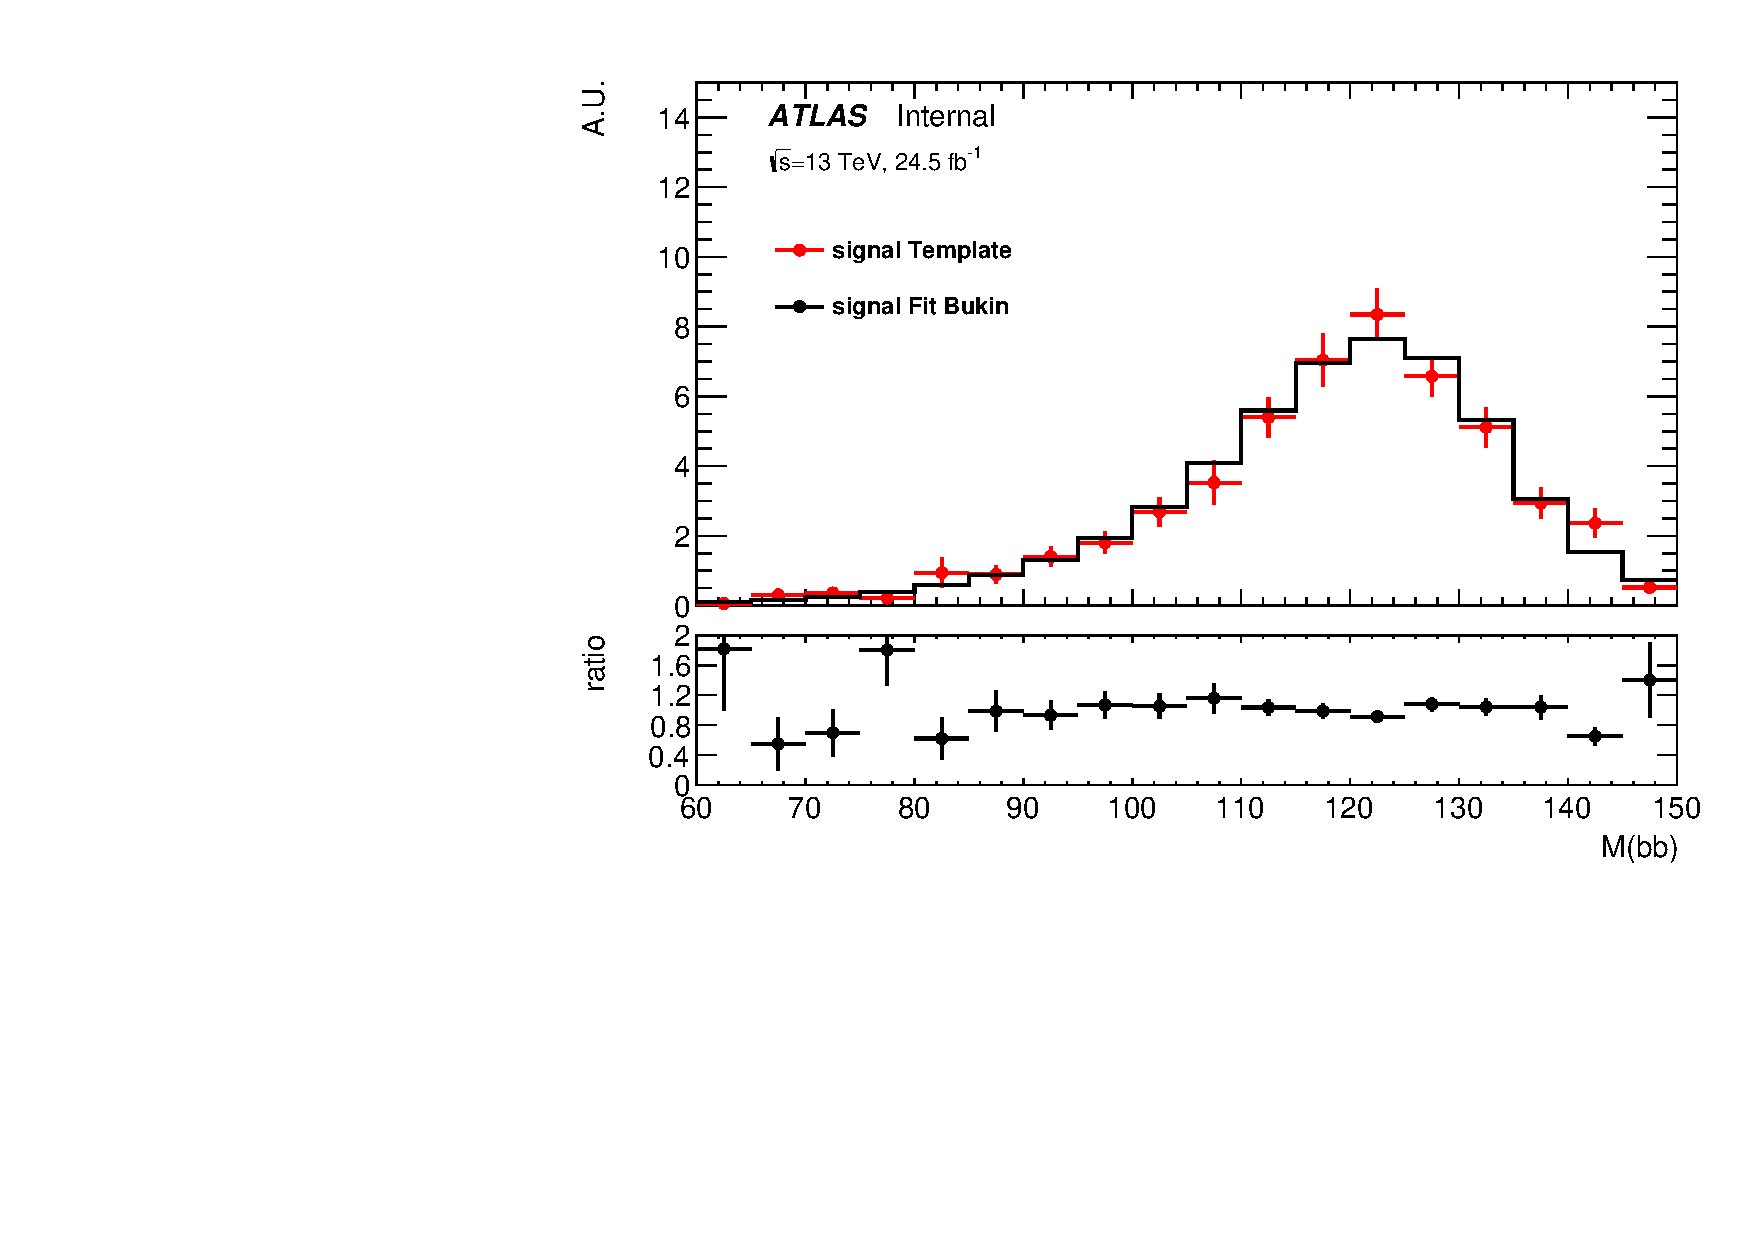
\includegraphics[width=0.24\textwidth]{figures/VBF/sig_4cen_SRII.pdf}
 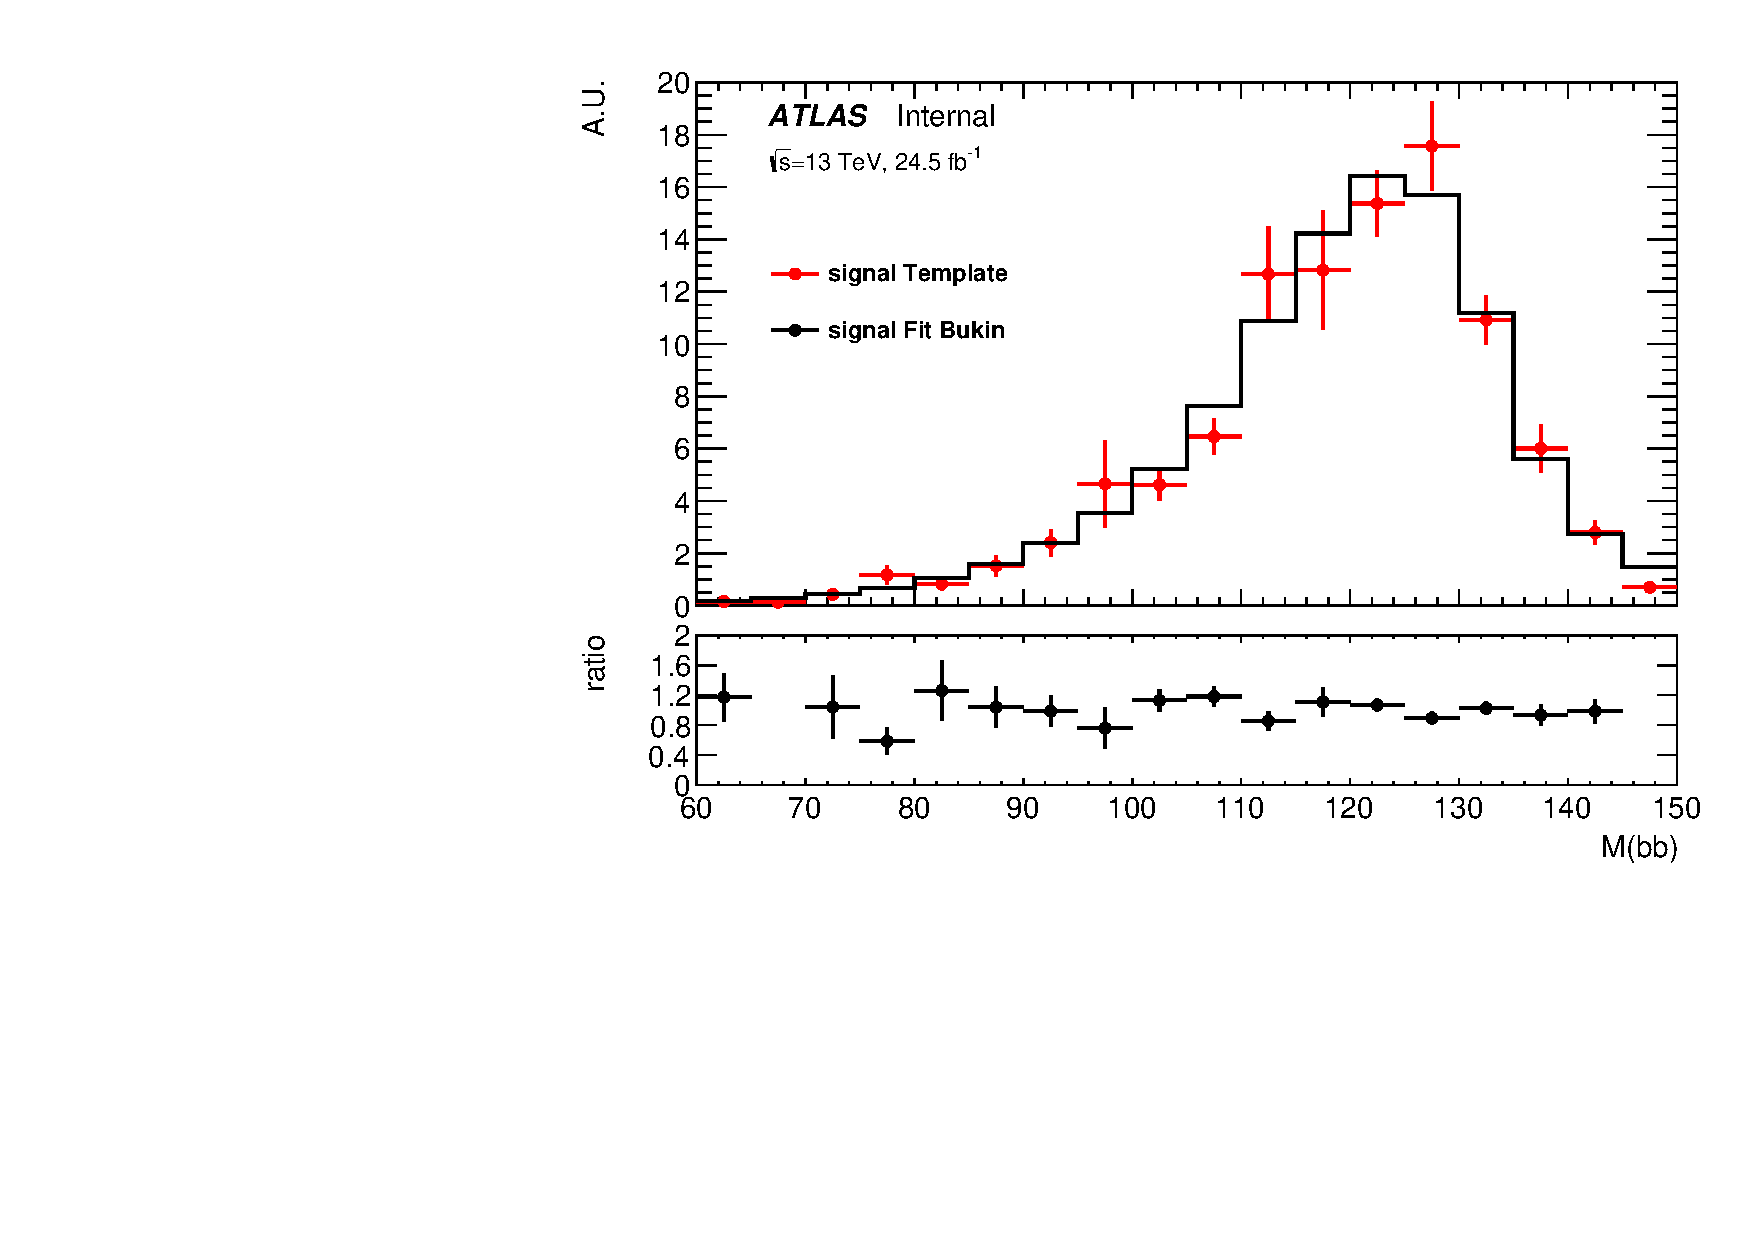
\includegraphics[width=0.24\textwidth]{figures/VBF/sig_4cen_SRIII.pdf}
 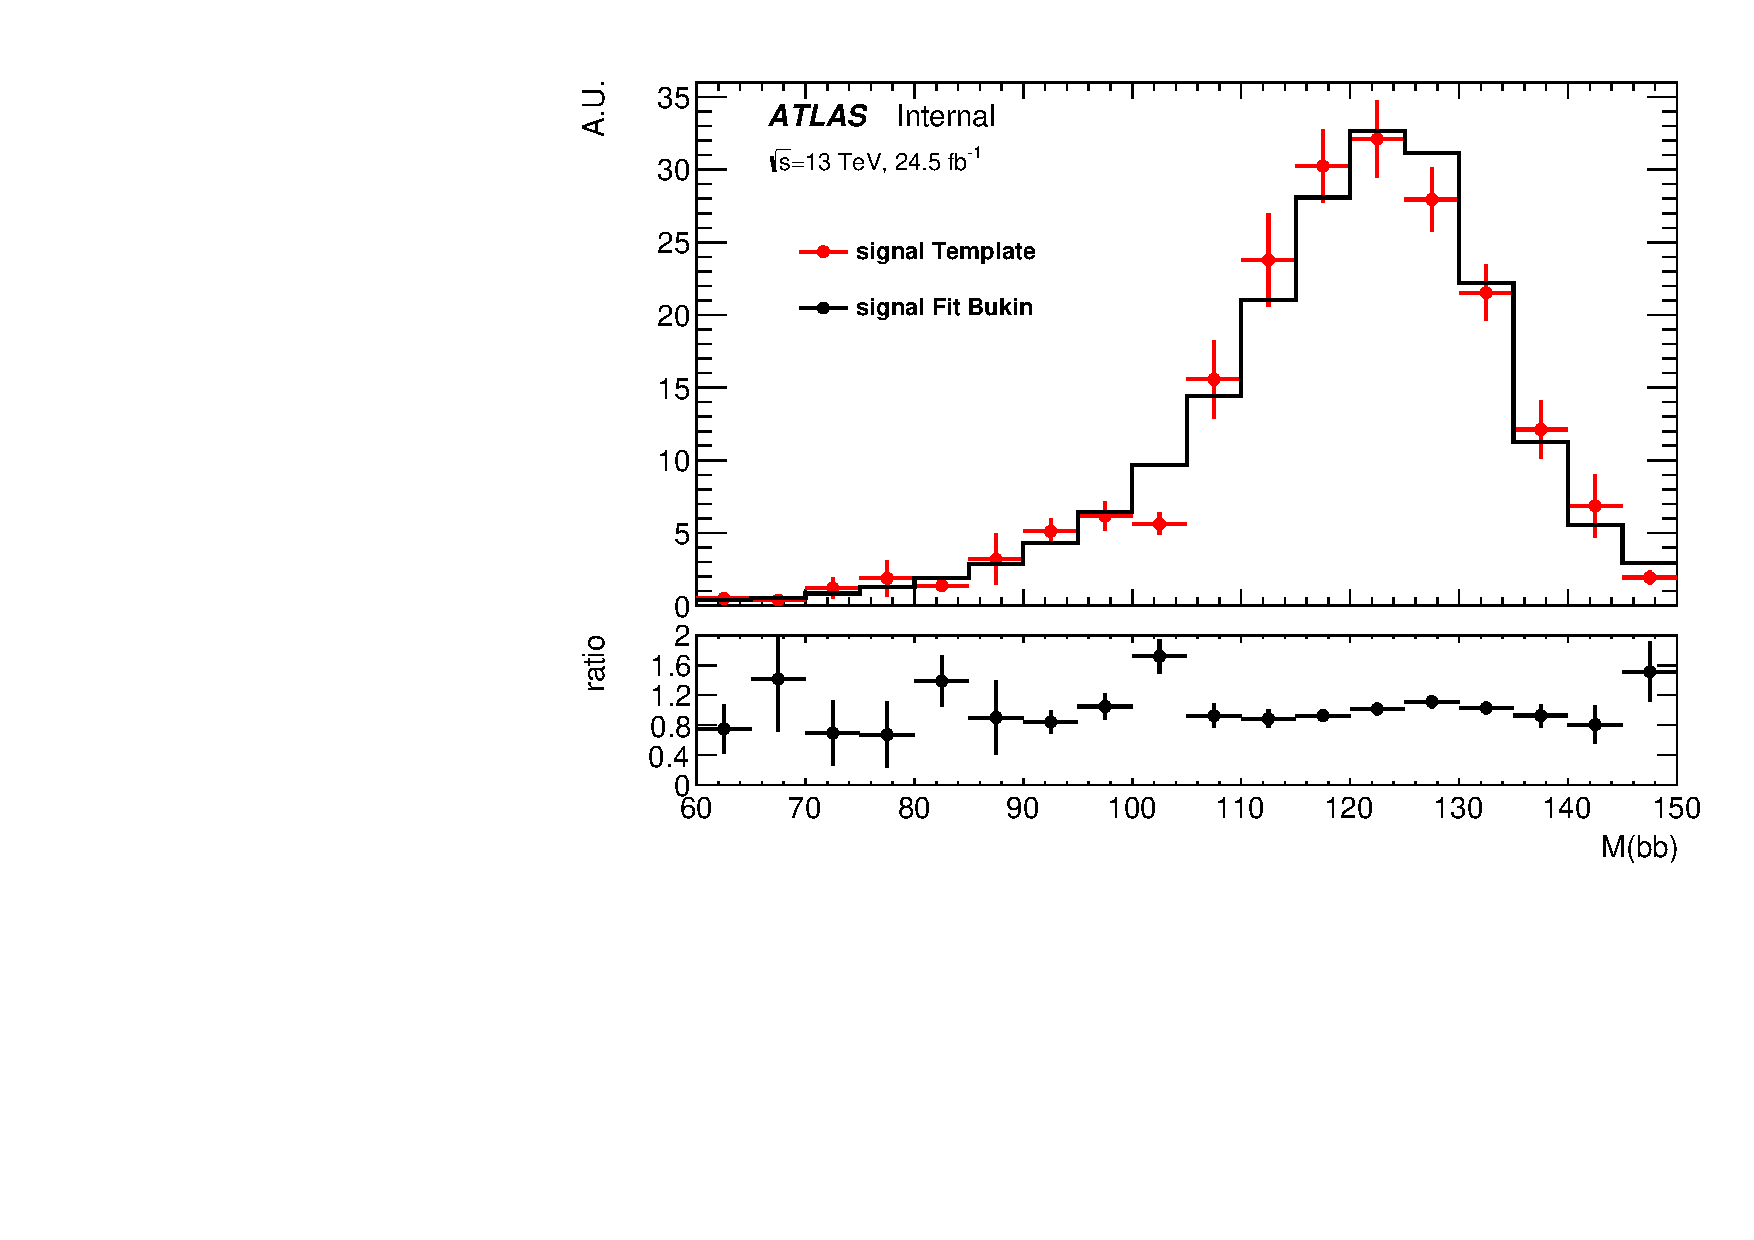
\includegraphics[width=0.24\textwidth]{figures/VBF/sig_4cen_SRIV.pdf}

\caption{Bukin function parametrization of signal \Mbb{} distributions of SR I to SR IV (left to right) in \twocentral (top) and \fourcentral (bottom) channels}
  \label{fig:vbf-sigpar_alt}
\end{figure}


\begin{figure}[htbp]
  \centering    
 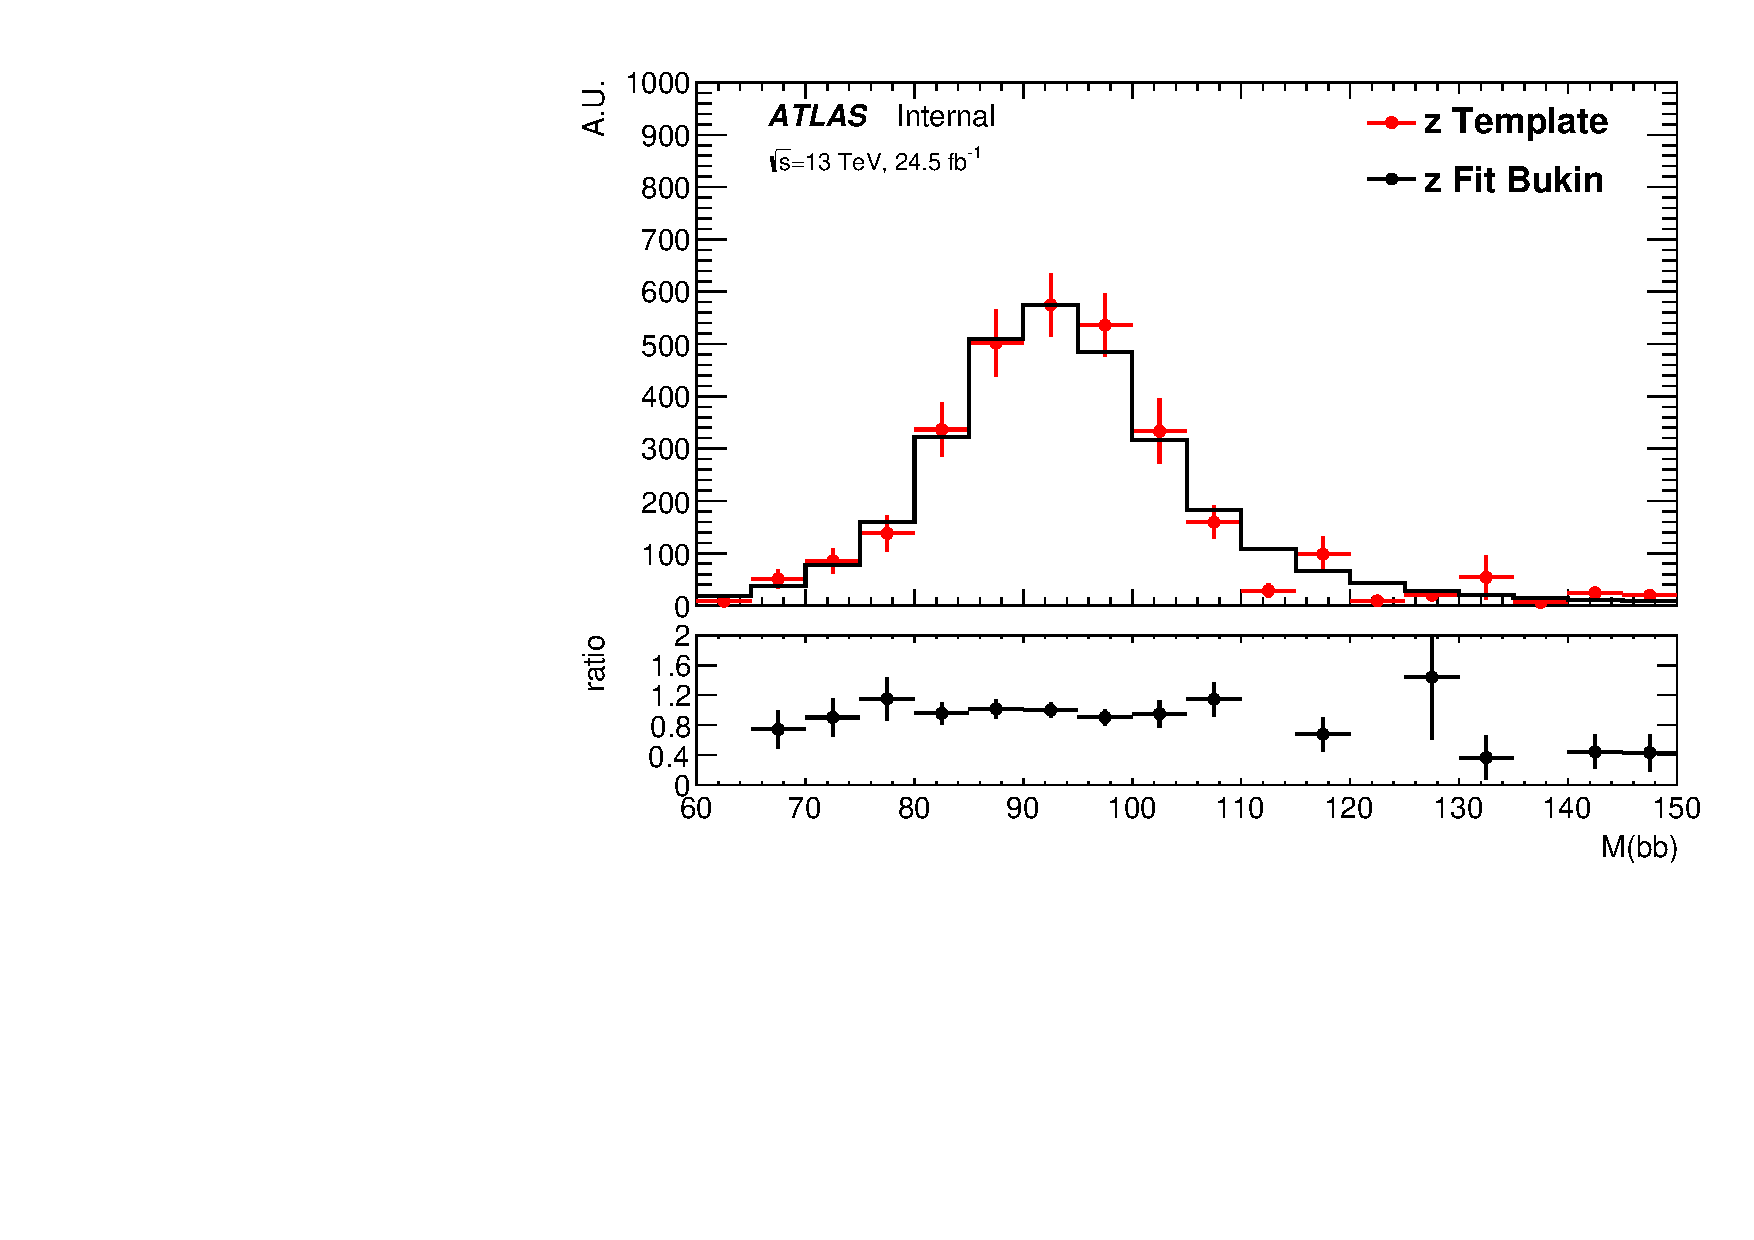
\includegraphics[width=0.45\textwidth]{figures/VBF/SigPar/z_2cen.pdf}
 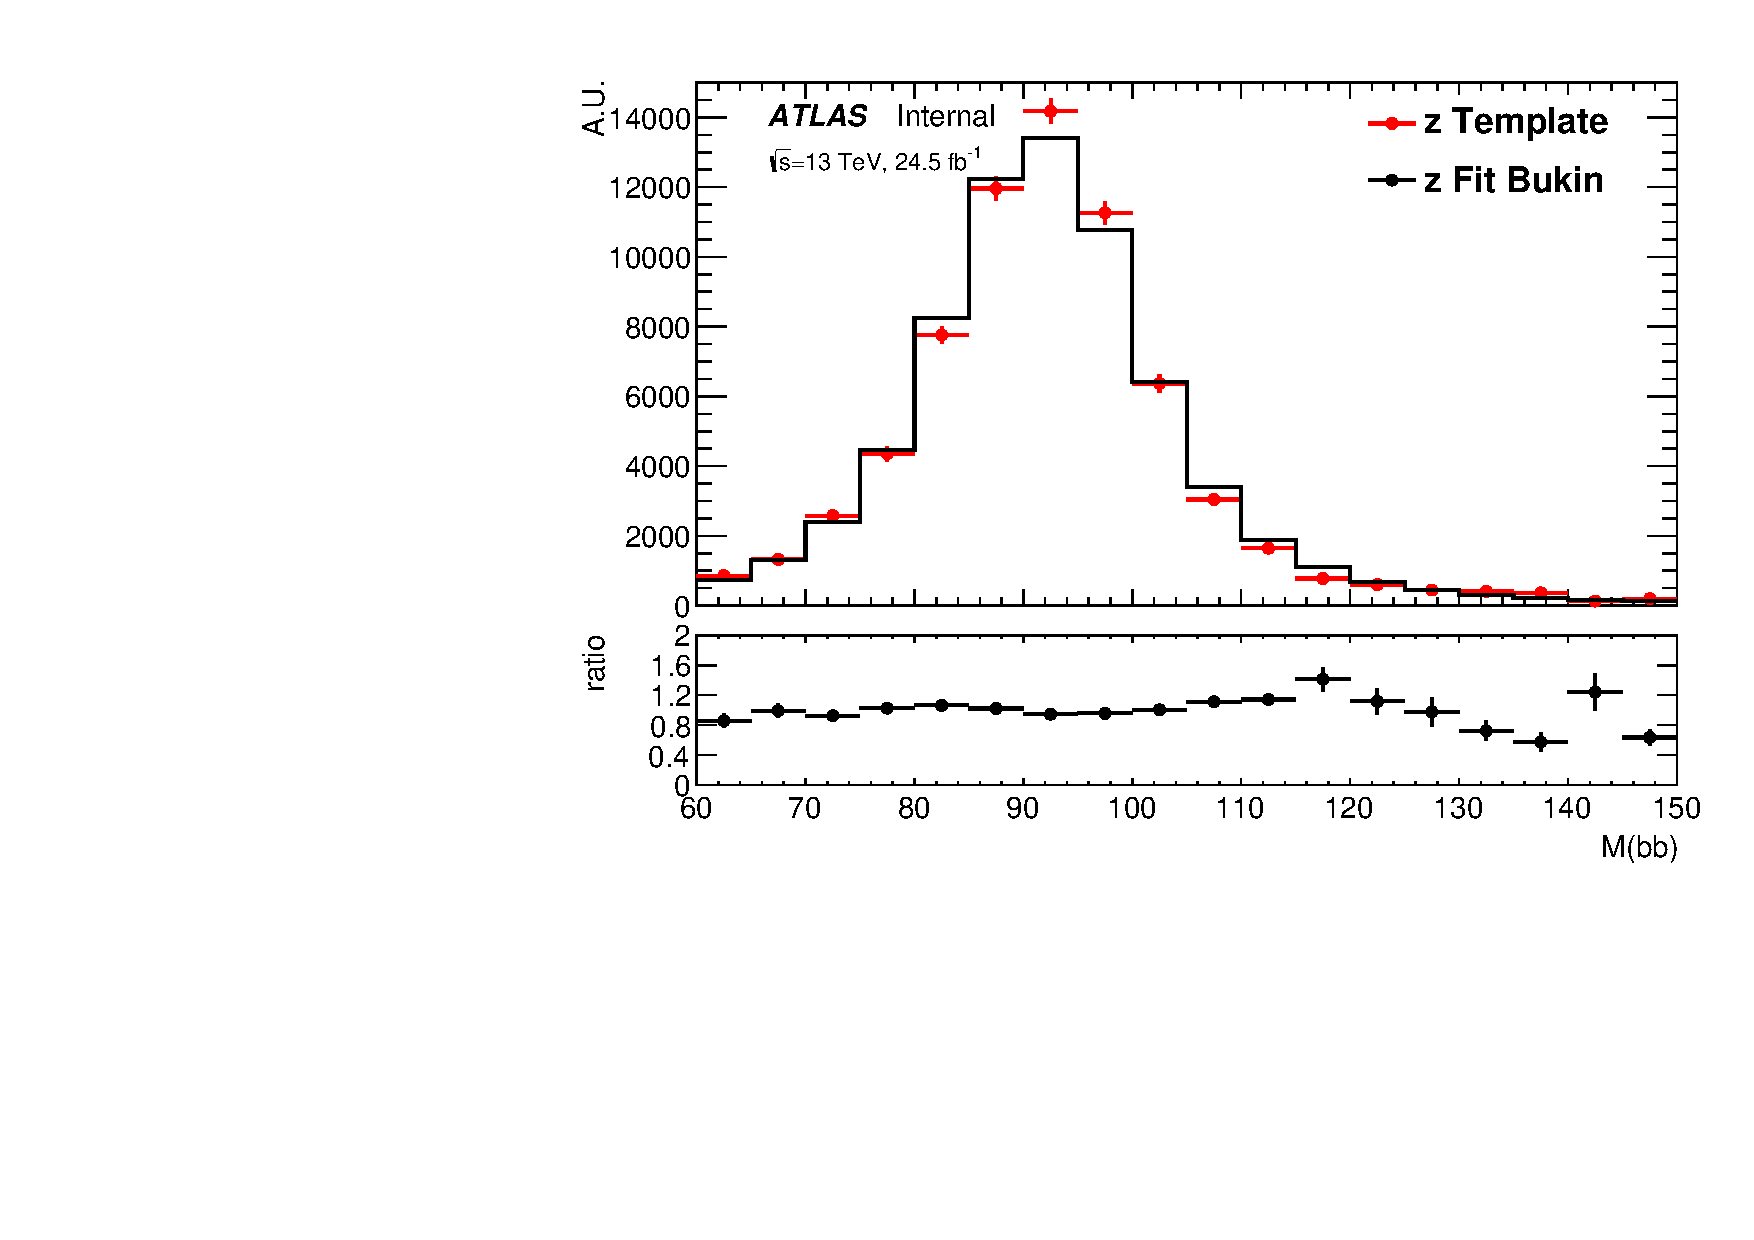
\includegraphics[width=0.45\textwidth]{figures/VBF/SigPar/z_4cen.pdf}

\caption{Bukin function parametrization of \zjets~\Mbb{} distribution in \twocentral (left) and \fourcentral (right). There are not enough events to divide the sample amongst BDT regions, therefore the distributions are shown for each channel preselection.}
\label{fig:vbf-zpar_alt}
\end{figure}


\begin{table}[htbp]
\centering
\caption{Goodness of fit for the Bukin parameterizations and signal and \zjets{} \Mbb{} distributions. There are not enough events for the \zjets{} sample to divide amongst BDT regions, therefore a the goodness of fit is shown for each channel preselection.}
\label{tab:sigpar_alt}
\begin{tabular}{|c|c|c|c|c|}
\hline
\multicolumn{5}{|c|}{$H\rightarrow b\bar b$ \fourcentral}                                                    \\ \hline
Region                                & \multicolumn{2}{c|}{SR I}        & \multicolumn{2}{c|}{SR II}        \\ \hline
\multicolumn{1}{|l|}{$\chi^2$ (Prob)} & \multicolumn{2}{c|}{0.85(0.64)}  & \multicolumn{2}{c|}{1.01(0.44)}   \\ \hline
\multicolumn{5}{|c|}{$H\rightarrow b\bar b$ \twocentral}                                                   \\ \hline
Region                                & SR I            & SR II          & SR III           & SR IV          \\ \hline
\multicolumn{1}{|l|}{$\chi^2$ (Prob)} & 1.06 (0.39)     & 0.77 (0.71)    & 1.10 (0.35)      & 1.21 (0.25)    \\ \hline
\multicolumn{5}{|c|}{\zjets}                                                                                 \\ \hline
Channel                               & \multicolumn{2}{c|}{\twocentral} & \multicolumn{2}{c|}{\fourcentral} \\ \hline
\multicolumn{1}{|l|}{$\chi^2$ (Prob)} & \multicolumn{2}{c|}{1.7 (0.04)}  & \multicolumn{2}{c|}{1.32 (0.17)}  \\ \hline
\end{tabular}
\end{table}


\subsubsection{Treatment of \zjets{} contribution}
\label{sec:vbf-ztreat}

The \zjets{} contribution plays an important role in the overall fitting procedure due to the fact that it comprises a significant fraction lower \Mbb{} sideband ( 1--7 (2--4)\% of the \fourcentral(\twocentral) selection), yet the sideband does not extend to low enough \Mbb{} values to reliably constrain its contribution using the shape templates.  Therefore, the non-resonant background fit can be partially compensated by the $Z$-yield and vice-versa.  To mitigate the impact of this degeneracy, we could fix the contributions of \zjets{} in the fits to predictions from MC.  However, our \zjets{} MC is only leading order ($Z+$2 partons), and large or varying $k$-factors may be present in the different BDT regions.  Therefore, we assume no prior knowledge of $Z$ contribution in all BDT regions and allow the contribution to float in the profile likelihood fit. This is the most conservative strategy and yields the largest decrease in overall sensitivity. Other strategies are investigated in Appendix~\ref{sec:vbf-app-zstrat}.

